\section{Digital Ownership within LAOS}\label{laos-assets}

LAOS Assets (LA) are Non-Fungible Tokens that can be created and evolved on the LAOS blockchain,
independent of the blockchain that manages their ownership. 
LA extend first-generation NFT technology by introducing the following features:
\begin{itemize}
    \item Bridgeless Connectivity: all aspects around ownership of an LA, including
    trading, lending, access to DeFi, etc., can be managed in any blockchain that supports smart contracts,
    while minting and evolution is managed in LAOS, without the need to resort to any type of bridge
    (technical details in Section \ref{sec:bridgeless-tech});
    \item Scalability. LA can be minted and evolved at scale, in fully decentralized flows;
    \item Full Decentralization. The attributes of all LA, now, and in every past state, can be certified on-chain, without 
    resorting to centralized privately-owned servers (technical details in Section \ref{sec:architecture}).
\end{itemize}

The following subsections provide a high-level overview of how these 
properties can be leveraged, focusing on the developers and users
point of view. The low-level technical
aspects are left for sections \ref{sec:architecture} and  \ref{sec:bridgeless-tech}.

\subsection{User Generated Value}\label{sec:ugv}

Scalability and the trust generated by the fact that 
mutability has a fully verifiable history are the key ingredients 
to one of the main paradigm shifts that LAOS Assets enable.

LA enable digital industries to migrate from a mindset of {\it scarcity} and {\it speculation},
to one of {\it abundance} and {\it User Generated Value} (UGV). In the latter, 
assets can be distributed at scale, at zero or very small initial value
(e.g., just for downloading and application or for signing-in), to a large base of users, hence 
eliminating all monetary entry barriers to owning a digital asset.

In this mindset of abundance, the initial market value of most assets is effectively zero.
DApps using LA can provide the flexibility to evolve based on both
off-chain activity (such as real-world events) and on-chain data.
By engaging with apps, video games,
online and social media activity, and the broader ecosystem,
LA owners can improve their assets (a more powerful game item,
an NFT that grants better rewards, an IP license granting further rights),
making them more valuable to others,
eventually converting their dedication, talent, and effort,
into increased market value.

\begin{Figure}
    \medskip
    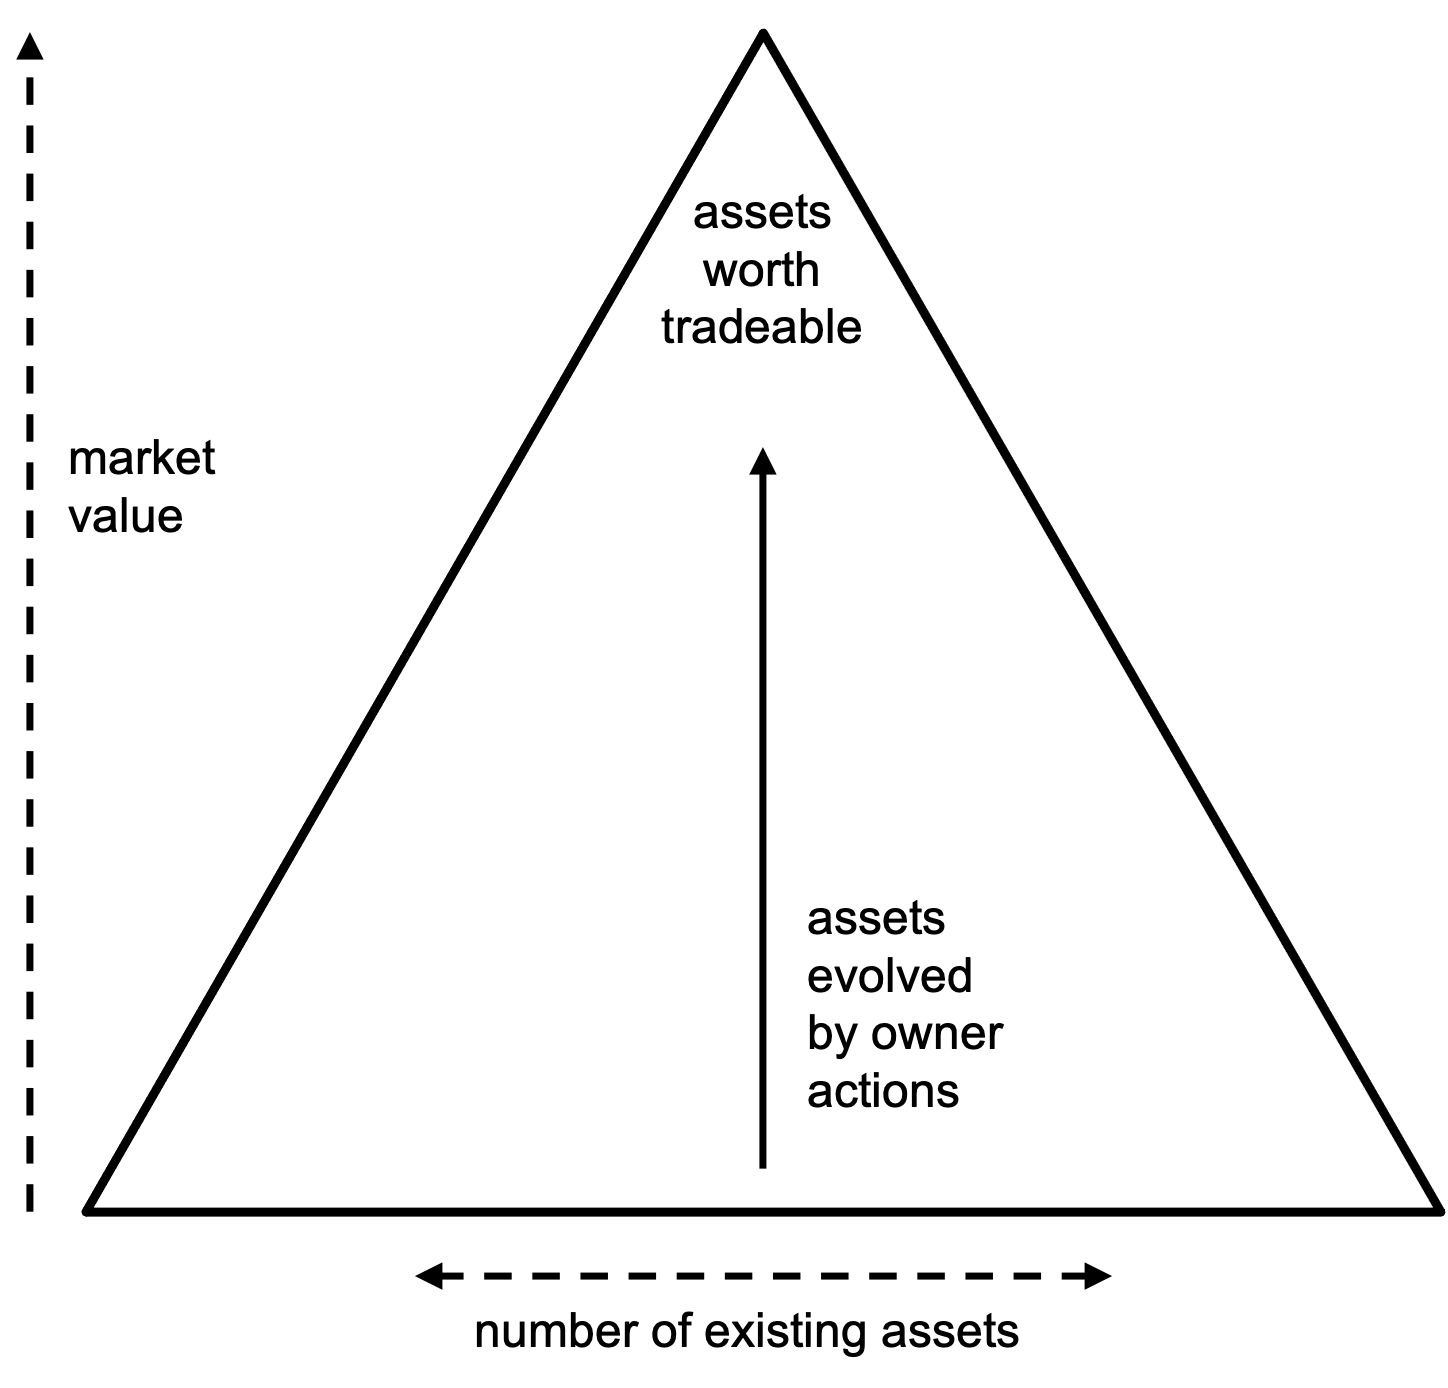
\includegraphics[width=1\textwidth]{pyramid.png}
    \captionof{figure}{
        Typical distribution of market value (y-axis) vs. 
        number of assets (width of the x-axis)
        in User Generated Value paradigms. A large number of assets with negligible market value 
        co-exist alongside a smaller percentage that have accrued significant value
        through the efforts of their owners.
    }
    \medskip
    \label{fig:pyramid}
\end{Figure}

UGV paradigms tend to reflect patterns common to Free-to-Play models
(Figure \ref{fig:pyramid}), whereby
a large base of assets with near-zero market value co-exist with further layers
of assets which users have evolved significantly with their actions. This pattern turns the 
sentiment of owning digital assets into an {\it active} experience, 
becoming a powerful engagement tool.


\subsection{Certifiability}\label{sec:ugv-certifiable}

UGV and the use cases mentioned in sections \ref{sec:la-bridglessness}-\ref{sec:use cases}
heavily rely on the history of the asset, on the confidence that NFTs have
market value accrued through a fair, traceable, set of evolutions.
It becomes paramount to be able to answer, in a fully trustless way, 
questions like {\it how did users turn this game item into something so powerful?}, or {\it how did
the owners of this NFT evolve it from scratch to an item with level-10 rewards?}

This is manifestly impossible in centralized flows derived from 
pattern \bref{eq:tokenURICentral}, since external privately-owned servers need 
to be trusted, exactly as in the pre-blockchain era.

LAOS provides the strongest forms of certifiability. On the one hand,
as described in Section \ref{sec:architecture}, all {\it data is fully available}
via decentralized flows, including data about the current and
past attributes of every asset.

On the other hand, LAOS enables any party to prove on-chain that an asset
with tokenId $id$ was in a certain state $s$ at any time $t$ in its history,
via the provision
of inclusion proofs $\Pi(id, s,t)$; these allow the blockchain to build {\it verify} 
methods which return true/false when queried:
\bea
\mbox{verify: \espai} id, s, t, \Pi(id, s,t) & \rightarrow & \mbox{bool}\,.
\eea

By virtue of LAOS being in the Polkadot ecosystem, it will be possible
to use these strong forms of certifiability as part of smart contract logic
built in other Parachains, such as Moonbeam\cite{moonbeam} or Astar\cite{astar}.
Example use cases would be contracts that allow owners of 
NFTs that have been evolved beyond a certain level to unlock certain rewards,
or that execute methods of a DeFi contract in the same blockchain.
An illustrative example of pseudo-code would be:
\begin{algorithm}[H]
    \KwData{Input values $id, s, t, \Pi(id, s,t)$}
    do initial logic\;
    \If{\textnormal{verify($id, s, t, \Pi$($id, s,t$))}}{
        do further logic based on $s,t$\;
    }
\end{algorithm}

Perhaps the simplest, yet powerful, example of this usage would be to enable {\it certified purchases}.
In this pattern, a buyer could sign a purchase transaction that is conditional on the asset
attributes, e.g., "buy this asset if and only if it has {\it level} larger than 100".

\subsection{Bridgeless Minting \& Evolution}\label{sec:la-bridglessness}

The scalable, strongly-certifiable, minting and evolution features of LAOS
can be added on top of the advantages that leading blockchains already
have in terms of mature ecosystems of users and DApps.

By means of example, we hereby discuss the use case of developers that
want to build applications which benefit both from LAOS features and
Ethereum's rich ecosystem of smart contracts and DApps.
Any other blockchain that supports Turing-complete
programming of smart contracts would work too. 

Developers only need to deploy once
an ERC721/1155 smart contract in Ethereum,
tuned to use the Universal Location pattern as described
in section \ref{sec:bridgeless-tech}. Next, they can mint and evolve
assets in that contract by simply executing the corresponding transactions in the 
LAOS blockchain. Anyone can permissionlessly, in a fully decentralized manner,
and without resorting to bridges, build new, or connect to existing,
marketplaces that operate with these assets by means of standard
ERC721/1155 calls on Ethereum.
In particular, this contract's assets can be connected, e.g., to smart contracts
in Ethereum that allow their rental or to fractionalize their ownership.

By doing so, applications can leverage paradigms where massive amounts
of assets are created in a scalable, certifiable way, in LAOS, with only
a small fraction of them having fairly accrued enough User Generated Value 
to be worth being traded in Ethereum.


\subsection{Use cases}\label{sec:use cases}

LAOS profoundly shifts traditional paradigms,
heralding new prospects for creators, users,
and industries at large.
Through its bridgeless connectivity,
it allows these new paradigms to emerge
within the most mature ecosystems currently available, including Ethereum.

By actively engaging with LA, owners wield the power
to shape and influence the attributes of their assets,
thereby directly impacting their intrinsic value.
This interactive participation fosters deeper connections between
users and their assets, transcending the conventional
notion of passive ownership.

The reimagining of digital ownership opens up
a wide range of compelling use cases.
With developers and their communities empowered by
new tools and increased flexibility,
it is impossible to predict the full extent of their
creative potential. Nevertheless, here are a few examples
that can be envisaged today.

{\bf Gaming.} Using LAOS bridgeless minting and evolution,
games can mint hundreds of millions of assets on Ethereum,
at minimal cost, allowing gamers to trade,
lend, and amplify their assets using Ethereum's vast applications. 

{\bf Legendary Collectibles.} Existing collections are given a
new lease of life, with their creators using LAOS to extend and evolve their initially static
image and metadata, e.g., creating seasonal campaigns.
Marketplaces and explorers show the past and current states easily,
ensuring the collection's year-round relevance and continued value.

{\bf Marketplaces.} Leading NFT marketplaces attract more users by
offering mass minting on Ethereum through no-code and API solutions.
They absorb the minimal gas costs
for all users meeting specific criteria and relays transactions to provide a gasless UX.

{\bf Interoperability.} Games boost user acquisition and retention
by letting players use assets from any blockchain.
Users pay for imports via in-app purchases, after which
the developer uses LAOS to permissionlessly extend metadata to match the game's
style and introduces new attributes that are evolved within the game.

{\bf DApps.} DApps protect themselves from legal issues regarding
their assets being considered securities,
by shifting their minting and evolution to LAOS.
Now, rather than using private servers, the assets
are stored securely on decentralized systems and can be verified on-chain.

{\bf User Generated Content.} LA allows the flourishing community of content generators to 
accrue market value to their talent and dedication. In a game or online 3D crafting app example,
users create a fully customized racing car, from engine tweaks, to paint job and looks,
and use LAOS' decentralized asset identity to incentivize games to import them and 
provide further utility.

{\bf Game Distribution Platforms.} Leading platforms partner with Copyright Offices
to enforce asset copyright across all blockchains, using LAOS' Decentralized Identity.



